
\section{Experiments}
\noindent\textbf{Dataset: Grid World.}~~
In this section, we first consider the discrete control environments from the Grid World \cite{14}, which is a commonly used benchmark for recent in-context RL methods. The environments support many tasks that cannot be solved through zero-shot generalization after pre-training because these tasks cannot be inferred easily from the observation. The episode of each task is short enough to train a transformer-based policy with across-episodic contexts feasibly. Specifically, we consider the four evaluation environments: Darkroom, Darkroom Hard, Darkroom Dynamic, and Dark Key-to-Door.

The evaluation environments provide a 2D discrete POMDP where an agent spawns in a room and must find a goal location. The agent only observes its own $(x,y)$ coordinates but does not know the goal location, which is required to deduce it from the rewards received. The room dimensions are $9\times9$ with the agent's possible actions, including moving one step either left, right, up, down, or staying idle. In Darkroom, an episode lasts 20 steps, and the agent can obtain a reward ($r=1$) each time the goal is achieved. The Darkroom Hard and Darkroom Dynamic are two variants of Darkroom. In the Darkroom Hard, agents only obtain a reward when the goal is achieved first. In the Darkroom Dynamic, the goal is fixed to a corner, but the action space is randomly permuted. In the Dark Key-to-Door, the length of an episode is 50, where the agent is required to locate an invisible key to receive a one-time reward first and then identify an invisible door to obtain another one-time reward.

In addition, we create a variant of Large Darkroom, Large Darkroom Hard, Large Darkroom Dynamic, and Large Darkroom Key-to-Door, where the coordinate space of each environment is expanded to $40\times40$, and the episode length is expanded 10 times. The dataset is collected from learning histories that are generated by training gradient-based RL algorithms, such as Deep Q-Network \cite{28}. For each environment, we randomly create 60 tasks from the coordinate space and collect data for 1 million timesteps. 

\begin{figure*}
    \centering
    
\includegraphics[width=1.8\columnwidth]{results/maze_results.pdf}
    \caption{Results for Grid World. An agent is expected to solve a new task by interacting with the environments for 50 episodes without online model updates. Based on high-level decisions, our method outperforms both AT and AD, which rely on across-episodic contexts with the smallest actions. In particular, IDT has significant advantages in handling long-horizon tasks.}
    \label{grid world}
\end{figure*}

\noindent\textbf{Dateset: D4RL.}~~
D4RL \cite{13} is a commonly used offline RL benchmark, including continuous control tasks. The different dataset settings are described below.

\begin{itemize}
    \item Medium: 1 million timesteps generated by a ``medium" policy that performs approximately one-third as well as an expert policy.
    \item Medium-Replay: 1 million timesteps collected from the replay buffer of an agent trained to the performance of a ``medium" policy.
    \item Medium-Expert: It consists of 1 million timesteps generated by the ``medium" policy and another 1 million timesteps generated by the expert policy.
\end{itemize}

The dataset is collected from Mujoco environments, including HalfCheetah, Hopper, and Walker. The episode length in D4RL is 1000, which is far more than that of Grid World. Therefore, current in-context RL methods require huge computational costs in D4RL, even though it is a commonly used baseline for conventional RL algorithms.




\noindent\textbf{Baselines.}~~
In this section, we investigate the performance and efficiency of IDT relative to in-context RL, dedicated offline RL, and imitation learning algorithms. Our baselines can be categorized as follows:

\begin{itemize}
    \item In-context RL: These methods use the transformer to model trajectory sequences and predict actions autoregressively. We compare with recent methods, Agentic Transformer (AT) \cite{1} and Algorithm Distillation (AD) \cite{8}, which proposed across-episodic contexts with the smallest actions.
    \vspace{-2pt}
    \item Temporal-difference learning: Most temporal-difference (TD) learning methods use an action space constraint or value pessimism and will serve as faithful comparisons to IDT, representing standard RL methods. We consider state-of-the-art TD3+BC \cite{29} that is demonstrated to be effective on D4RL.
    \vspace{-2pt}
    \item Imitation learning: Imitation learning methods similarly utilize supervised losses for training, such as Behavior Cloning (BC) \cite{30} and Decision Transformer (DT) \cite{2}. Following AT, we compare with BC-10$\%$, which is shown to be competitive with state-of-the-art on D4RL. DT also uses a transformer to predict actions autoregressively but is limited to a single episode context.
\end{itemize}

For all comparison methods, we adhere closely to the original hyper-parameter settings. To evaluate IDT and other in-context RL algorithms, we roll out 10 episodes in D4RL and 50 episodes in Grid World. For each result, we report mean and standard error across 5 random seeds.


\subsection{Evaluation of Computing Costs}
An important property of in-context RL is that it can improve itself without expensive gradient updates. However, the computational costs of forward propagation are hidden in short-horizon tasks. Therefore, we reported the training time per 10k gradient updates, the evaluation time for 50 episodes over Grid World, and 10 episodes over D4RL. As shown in Figure~\ref{cost_figure}, our IDT has efficient training and significantly reduces the testing time compared to the baselines, approximately \textbf{36$\bm\times$} times faster in D4RL and \textbf{27$\bm\times$} times faster in large Grid World. More detailed results for each task are described in Appendix~\ref{additional experiments}.

As the task length increases, the evaluation time of AT and AD grows quadratically.
This is because the across-episodic contexts multiply the sequence length, leading to intolerable computational costs in the self-attention mechanism. The AT algorithm requires four episodes for trial-and-error, where each episode reaches 1000 steps in D4RL, and each step contains 5 tokens. 
Therefore, each step of AT generation requires scanning 20k tokens.
Since the AD algorithm reduces a return-to-go token at each step, the training and testing time are both less than AT.
In contrast, IDT reconstructs the sequence to consist of high-level decisions, and thus, the context is smaller than one episode length. As a result, IDT is significantly lower than baselines at both training and testing times.


\begin{table*}
\caption{Results for D4RL datasets. IDT outperforms both in-context RL (AT and AD) and supervised learning (BC) and performs competitively with conventional RL algorithms (TD3+BC and TD3) on almost all tasks.
% The cumulative rewards demonstrate that our SGFD model generalizes well to new values of task-irrelevant features. 
}
\begin{center}
\resizebox{0.95\textwidth}{!}{
\begin{tabular}{lr|rrrrrrr}
\toprule
\specialrule{0em}{1.0pt}{1.0pt}
\toprule
Dataset & Environment & BC-10$\%$ & TD3+BC & TD3 & DT & AT & AD& Ours \\ 
\toprule
Medium-Expert & HalfCheetah & 94.11 & \textbf{96.59} & 87.60 & 93.40 & 95.81\scriptsize{$\pm$ 0.25} & 94.21 \scriptsize{$\pm$ 0.46} & 96.12\scriptsize{$\pm$ 0.18} \\ 
Medium-Expert & Hopper & 113.13 & 113.22 & 98.41 & 111.18 & 115.92\scriptsize{$\pm$ 1.26} & 108.32 \scriptsize{$\pm$ 0.95} & \textbf{118.39\scriptsize{$\pm$ 0.75}} \\ 
Medium-Expert & Walker & 109.90 & 112.21 & 100.52 & 108.71 & 114.87\scriptsize{$\pm$ 0.56} & 111.36 \scriptsize{$\pm$ 0.46}& \textbf{118.51\scriptsize{$\pm$ 0.48}} \\ 
\toprule
Medium & HalfCheetah & 43.90 & \textbf{48.93} & 34.60 & 42.73 & 45.12\scriptsize{$\pm$ 0.34} & 42.28 \scriptsize{$\pm$ 1.18} & 45.51\scriptsize{$\pm$ 0.26} \\ 
Medium & Hopper & 73.84 & 70.44 & 56.98 & 69.42 & 70.45\scriptsize{$\pm$ 0.45} & 72.58 \scriptsize{$\pm$ 0.54} & \textbf{83.24\scriptsize{$\pm$ 0.33}} \\ 
Medium & Walker & 82.05 & 86.91 & 70.95 & 74.70 & 88.71\scriptsize{$\pm$ 0.55} &85.96 \scriptsize{$\pm$ 0.46} & \textbf{88.94\scriptsize{$\pm$ 0.61}} \\ 
\toprule
Medium-Replay & HalfCheetah & 42.27 & 45.84 & 38.81 & 40.31 & \textbf{46.86\scriptsize{$\pm$ 0.33}} & 41.28 \scriptsize{$\pm$ 0.21} & 45.58\scriptsize{$\pm$ 0.36}\\ 
Medium-Replay & Hopper & 90.57 & 98.12 & 78.90 & 88.74 & 96.85\scriptsize{$\pm$ 0.41} &91.32 \scriptsize{$\pm$ 0.66} & \textbf{98.59\scriptsize{$\pm$ 0.26}} \\ 
Medium-Replay & Walker & 76.09 & 91.17 & 65.94 & 68.22 & 92.32\scriptsize{$\pm$ 1.21} & 89.21 \scriptsize{$\pm$ 1.42}& \textbf{96.22\scriptsize{$\pm$ 1.06}} \\
\toprule
\multicolumn{2}{c|}{Total Average} & 80.65\scriptsize{$\pm$ 1.34} & 84.83\scriptsize{$\pm$ 1.10} & 70.28\scriptsize{$\pm$ 1.20} & 77.49\scriptsize{$\pm$ 1.45} & 85.21\scriptsize{$\pm$ 1.12} & 82.84\scriptsize{$\pm$ 0.70} & \textbf{87.90\scriptsize{$\pm$ 1.06}}\\
\toprule
\specialrule{0em}{1.0pt}{1.0pt}
\toprule
\end{tabular}
}
\end{center}
\label{d4rl}
\end{table*}

\begin{figure}
    \centering
    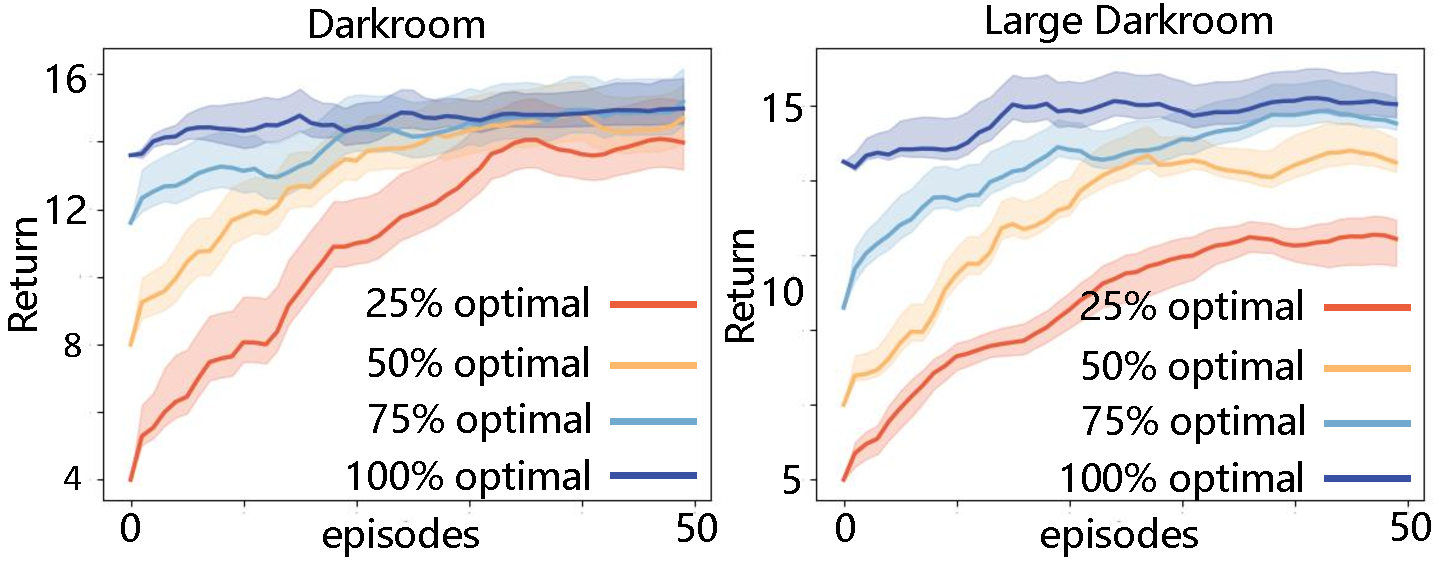
\includegraphics[width=0.85\columnwidth]{results/promt_results.pdf}
    \caption{Results for IDT conditioned on partial demonstrations. IDT can accelerate self-improvement through the Review Decisions module to encode external data prompts. 
    % When the external data provided is closer to optimal experts, IDT can solve the evaluation task directly.
    }
    \label{partial demonstrations}
\end{figure}

\subsection{Grid World Results}
To evaluate IDT’s self-improvement capabilities in unseen tasks, we compared recent in-context RL methods in the Grid World environments. The agent is required to solve an unseen task by interacting with the environments for 50 episodes without online model updates. As shown in Figure~\ref{grid world}, IDT achieves state-of-the-art performance in a wide range of tasks.

In large variant tasks, IDT significantly surpasses the baselines in both efficiency and performance. However, neither AT nor AD showed obvious self-improvement trends, especially in Large Darkroom Hard. This is because the Large Darkroom Hard is a task with sparse rewards, which makes it difficult for AT and AD to capture the goal position in long sequences. In contrast, IDT explores tasks in a high-level trial-and-error manner, making receiving positive feedback on rewards easier. Overall, IDT demonstrated that a high-level trial-and-error manner is feasible rather than limited to the smallest actions.

% Overall, IDT provides a new idea for in-context RL methods, showing that a high-level trial-and-error manner is feasible rather than limited to the smallest actions.

\subsection{D4RL Results}
In addition to short-horizon tasks specific to in-context RL methods, we also test the performance of IDT on the D4RL dataset, which is commonly used in conventional RL methods. Based on \citet{13}, the results on D4RL are normalized so that 100 denotes an expert policy. Baseline numbers are reported by the AT paper and from the D4RL paper.
As shown in Table~\ref{d4rl}, IDT outperforms baselines in a majority of the tasks and is competitive with the state-of-the-art in the remaining tasks.

In the TD learning and imitation learning categories, TD3+BC is generally the most remarkable algorithm. Compared with them, the superior performance of IDT demonstrates the advantages of using high-level trial-and-error.


\subsection{Case Study on the Reviewing Decisions Module}
A notable ability of transformer-based policy is to address tasks by providing demonstration prompts. Although in-context RL can improve itself without relying on demonstrations, external prompts can speed up the process.
Therefore, we want to investigate whether IDT can benefit from this setting. 
To answer this question, we design a $\epsilon$-greedy policy to collect external data in Darkroom and Large Darkroom tasks, ranging from nearly random to optimal.

As shown in Figure~\ref{partial demonstrations}, IDT improves each policy in context until it is near-optimal. Notably, the more optimal the input policy, the faster IDT improves it until it is optimal. Despite high-level decisions that cannot be directly observed from the external demonstrations, IDT can extract experts' intentions through the Reviewing Decisions module. In particular, we also perform parameter sensitivity analyses on high-level decision frequency ($c$) and context size ($n$ episodes), as shown in Appendix~\ref{additional experiments}.



